\documentclass[letterpaper,10pt]{article}
\title{Assignment 4 Report - Kmeans and Clustering}
\author{Helena Bales and Natalie Suderman\\ \\ CS434 - Spring 2017}
\usepackage[pdftex]{graphicx}
\usepackage{tikz}
\usepackage{float}

\parindent = 0.0 in
\parskip = 0.1 in

\begin{document}
\maketitle

\tableofcontents
\clearpage

%%\section{Introduction}

\section{Non-Hierachical Clustering Implementing K-means algorithm}

\subsection{Implementing K-means with K of 2}
	The results of  typical run of the kmeans algorithm when k is 2. I plotted multiple runs to show the trend.
     \begin{figure}[ht]
    \centering
   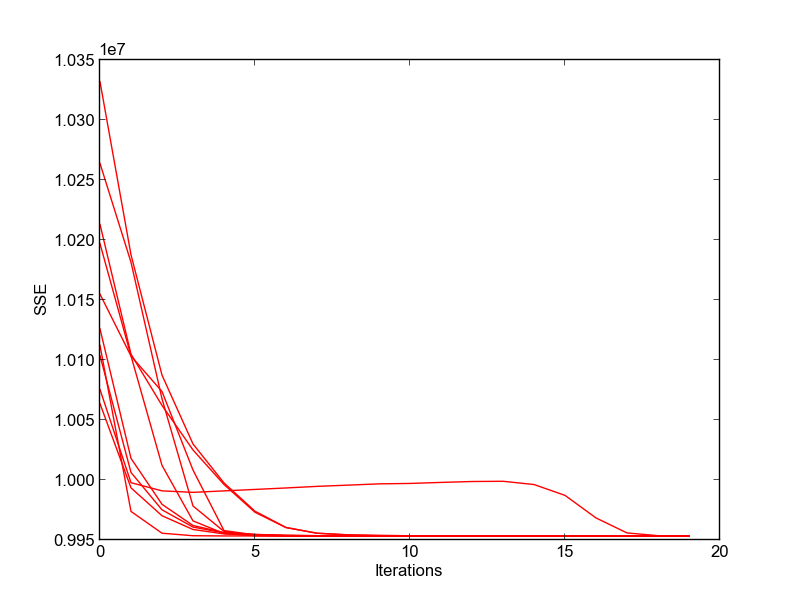
\includegraphics[width=300pt]{k2means.png}
    \caption{A typical run. SSE of Kmeans with k of 2 over number of iterations.}
    \label{fig:k2}
    \end{figure}	

\subsection{Apply K means to different values of K}
The algorithm was tested by using different values of K (3, 4, 10, etc) 
and the minimum SSE from 10 runs for each K was plotted to demonstrate 
a trend in the size of the SSE vs number of K. 

     \begin{figure}[ht]
    \centering
   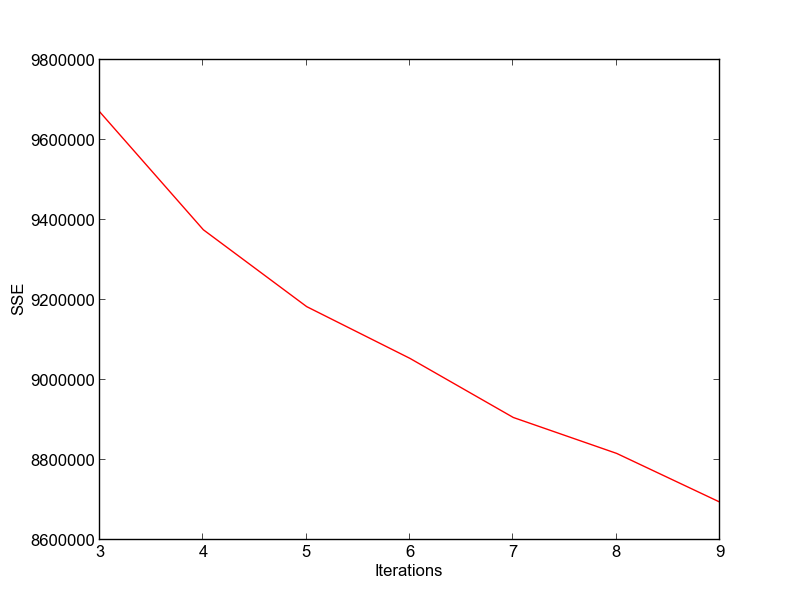
\includegraphics[width=300pt]{diffks.png}
    \caption{Min SSE found over 10 runs of the algorithm for each k tested.}
    \label{fig:diffk}
    \end{figure}	


\section{Hierarchical Agglomerative Clustering}
\subsection{Compute HAC Using Single Link}
     \begin{figure}[ht]
    \centering
   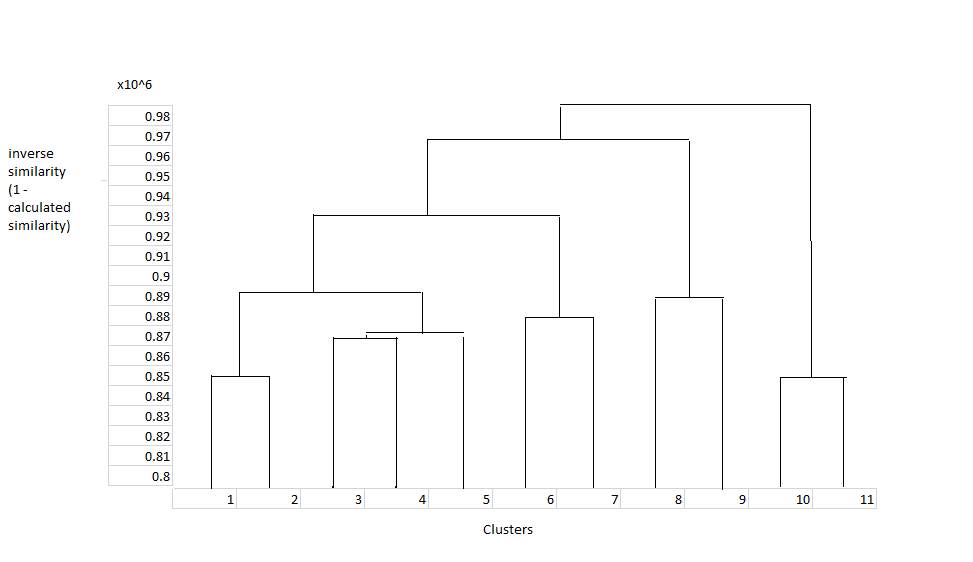
\includegraphics[width=300pt]{dendroHAC.png}
    \caption{Dendrogram starting with 10 clusters. Difference/height is reported as an inverse of similarity. ie. Higher similarity calculated equals lower difference/height of dendrogram}
    \label{fig:diffk}
    \end{figure}	

	similarities reported: 
	(1,2) 1499919.0
	(3,4) 1208826.0
	(3,4,5) 1207976.0
	(6,7) 1127700.0
	(8,9) 1065419.0
	(1,2,3,4,5) 1057888.0
	(1,2,3,4,5,6,7) 632494.0
	(1,2,3,4,5,6,7,8,9) 280324.0
	(10,11) 1489698.0

\subsection{Compute HAC Using Complete Link}


\end{document}
